\clearpage
\section{Casi d'uso}
\subsection{Attori dei casi d'uso}
\subsubsection{Attori primari}
%immagine gerarchio utilizzo + didascalia
\begin{itemize}
	\item  Utente generico: utente che, indipendentemente dal fatto che abbia effettuato il login o meno, accede all'applicazione;
	\item  Utente non autenticato: utente che non ha effettuato il login;
	\item  Utente autenticato: utente che ha completato la procedura di autenticazione.
\end{itemize}

%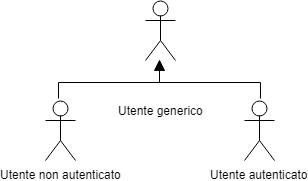
\includegraphics[width=1\textwidth]{../includes/pics/primari.png}
\begin{figure}[H]
	\centering
	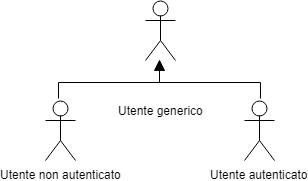
\includegraphics[width=10cm,keepaspectratio]{../includes/pics/primari.png}
	\caption{\label{fig:mission}Utenti del sistema}
\end{figure}

\subsection{Elenco dei casi d'uso}
%immagine attori che accedono a casi d'uso+didascalia

%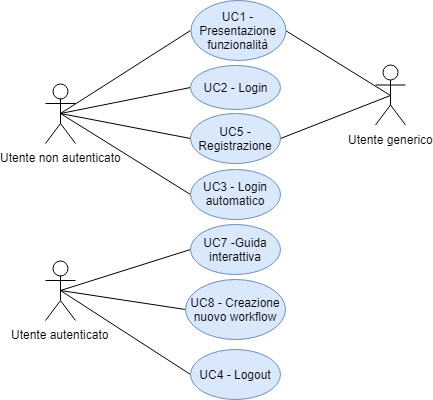
\includegraphics[width=1\textwidth]{../includes/pics/azioni_attori.png}
\begin{figure}[H]
	\centering
	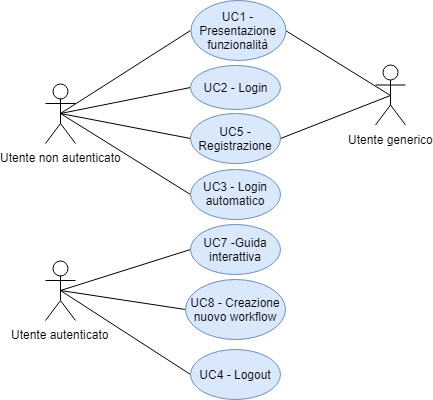
\includegraphics[width=10cm,keepaspectratio]{../includes/pics/azioni_attori.png}
	\caption{\label{fig:mission}Casi d'uso basilari per i vari utenti}
\end{figure}

\subsubsection{UC1 - Presentazione funzionalità}
\begin{itemize}
	\item  Attori primari: utente generico;
	\item  Scopo e descrizione: viene presentato all'utente una breve guida illustrata che permette di capire cosa è possibile fare con l'applicazione;
	\item  Scenario principale: l'utente visualizza la presentazione;
	\item  Pre-condizione: il sistema è funzionante e raggiungibile;
	\item  Post-condizione: l'utente è stato informato di alcune abilità del sistema.
\end{itemize}

%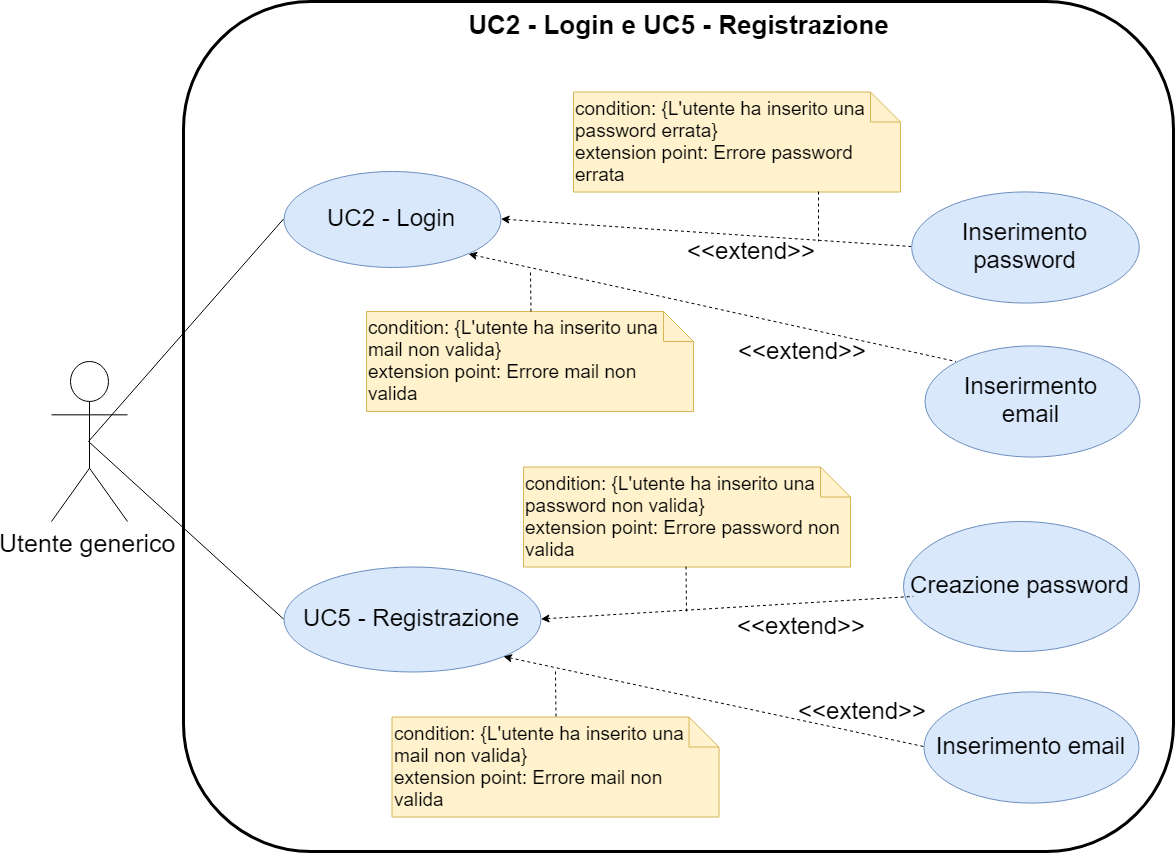
\includegraphics[width=1\textwidth]{../includes/pics/login_e_registrazione.png}
\begin{figure}[H]
	\centering
	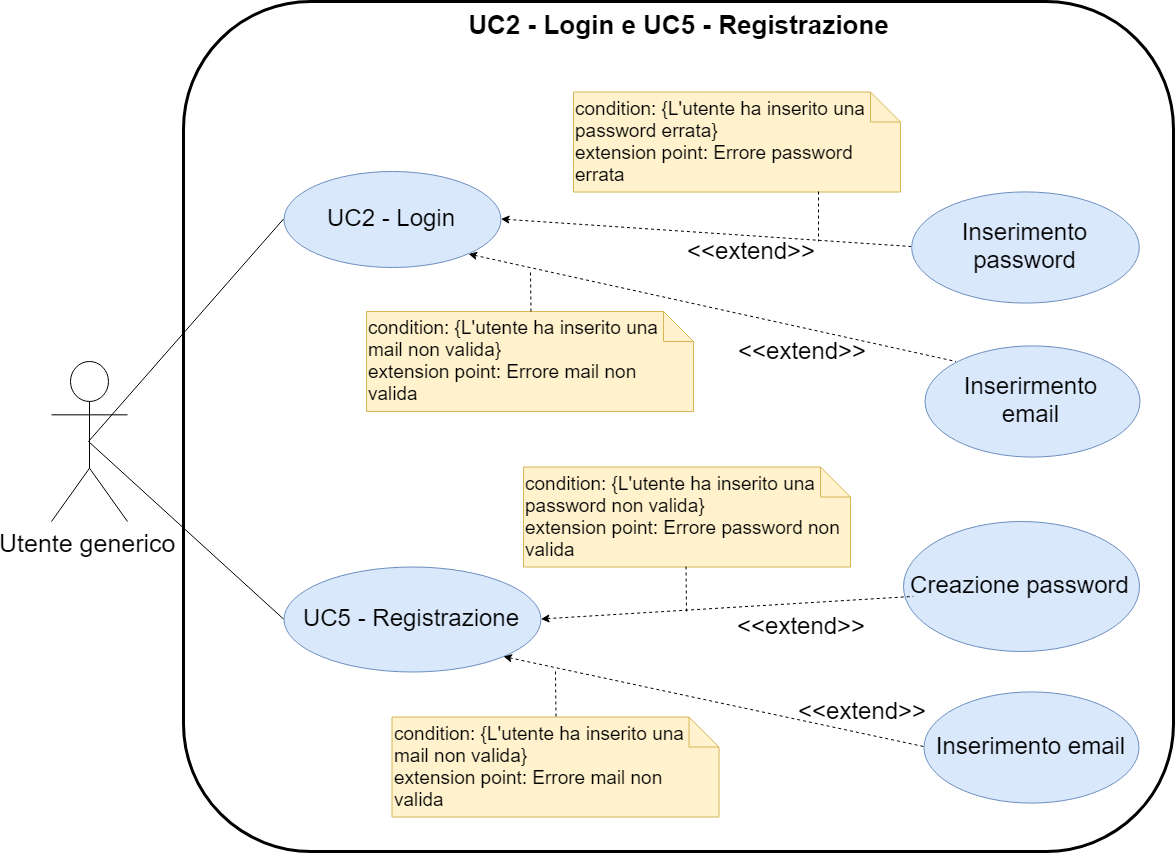
\includegraphics[width=15cm,keepaspectratio]{../includes/pics/login_e_registrazione.png}
	\caption{\label{fig:mission}Casi d'uso per login e registrazione}
\end{figure}

\subsubsection{UC2 - Login}
\begin{itemize}
	\item  Attori primari: utente non autenticato;
	%Attore secondario : \markg{server} che gestisce i dati utente (aws?)
	\item  Scopo e descrizione: viene presentato un form che permette all'utente di inserire le proprie credenziali necessarie per l'autenticazione;
	\item  Scenario principale: l'utente esegue la procedura di autenticazione;
	\item  Estensioni:
		   \begin{itemize}
				\item se l'utente inserisce una mail non valida, oppure non registrata nel sistema, riceve un messaggio di errore [UC2.1];
				\item se l'utente inserisce una password non valida riceve un messaggio di errore [UC2.2];
				\item se il \markg{server} di autenticazione non è raggiungibile, l'utente riceve un messaggio di errore di connessione [UC2.3].
		   \end{itemize}
	\item  Pre-condizione: l'utente non è autenticato;
	\item  Post-condizione: l'utente è autenticato, viene riconosciuto dal sistema e accede alla sua bacheca.
\end{itemize}
\subsubsection{UC2.1 - Visualizzazione messaggio errore mail identificativa}
\begin{itemize}
	\item  Attori primari: utente non autenticato;
	\item  Scopo e descrizione: l'utente viene avvisato che la mail inserita non identifica alcun account registrato;
	\item  Scenario principale: l'utente visualizza l'errore relativo all'errato inserimento della mail;
	\item  Pre-condizione: l'utente richiede il login inserendo una mail non valida oppure non registrata nel sistema;
	\item  Post-condizione: l'utente è consapevole di dover fornire una mail registrata e valida.
\end{itemize}
\subsubsection{UC2.2 - Visualizzazione messaggio errore password non valida}
\begin{itemize}
	\item  Attori primari: utente non autenticato;
	\item  Scopo e descrizione: l'utente viene avvisato che la password inserita non è associata alla mail inserita;
	\item  Scenario principale: l'utente visualizza l'errore relativo all'errato inserimento della password;
	\item  Pre-condizione: l'utente esegue il login inserendo una password errata;
	\item  Post-condizione: l'utente è consapevole di dover fornire una password associata alla mail inserita.
\end{itemize}
\subsubsection{UC2.3 - Visualizzazione messaggio errore connessione al \markg{server} di autenticazione}
\begin{itemize}
	\item  Attori primari: utente non autenticato;
	\item  Scopo e descrizione: l'utente viene avvisato che non è possibile comunicare con il \markg{server} di autenticazione a causa di un errore di connessione;
	\item  Scenario principale: l'utente visualizza l'errore relativo alla mancanza di una connessione stabile;
	\item  Pre-condizione: l'utente richiede il login senza avere una connessione internet, oppure il \markg{server} di autenticazione non è momentaneamente raggiungibile;
	\item  Post-condizione: l'utente è consapevole di dover fornire una connessione internet all'applicazione.
\end{itemize}
\subsubsection{UC3 - Login automatico}
\begin{itemize}
	\item  Attori primari: utente non autenticato;
	%Attore secondario : \markg{server} che gestisce i dati utente (aws?)
	\item  Scopo e descrizione: l'utente attende che il sistema lo autentichi con dati inseriti in precedenza e salvati nel dispositivo;
	\item  Scenario principale: l'utente viene riconosciuto dal sistema senza che gli vengano richiesti i dati di accesso;
	\item  Pre-condizione: l'utente non è autenticato;
	\item  Post-condizione: l'utente è autenticato, viene riconosciuto dal sistema e accede alla sua bacheca.
\end{itemize}
\subsubsection{UC4 - Logout}
\begin{itemize}
	\item  Attori primari: utente autenticato;
	%Attore secondario : \markg{server} che gestisce i dati utente (aws?)
	\item  Scopo e descrizione: l'utente tramite opportuno comando termina la propria sessione con l'applicazione;
	\item  Scenario principale: l'utente effettua la procedura di de-autenticazione;
	\item  Pre-condizione: l'utente è autenticato e riconosciuto dal sistema;
	\item  Post-condizione: l'utente non è più autenticato e viene riportato al form di login [UC2].
\end{itemize}
\subsubsection{UC5 - Registrazione}
\begin{itemize}
	\item  Attori primari: utente non autenticato;
	%Attore secondario : \markg{server} che gestisce i dati utente (aws?)
	\item Scopo e descrizione: l'utente non autenticato può scegliere se compilare i campi richiesti dalla form di registrazione, oppure registrarsi tramite associazione ad account \markg{Google} [UC5.2] o \markg{Amazon} [UC5.3];
	\item  Scenario principale: l'utente inserisce i propri dati personali e riceve l'autenticazione;
	\item  Estensioni: 
		   \begin{itemize}
				\item se l'utente inserisce una mail già registrata riceve un messaggio di errore [UC5.1.1];
				\item se l'utente inserisce una password non valida riceve un messaggio di errore [UC5.1.2];
				\item se il \markg{server} di autenticazione non è raggiungibile, l'utente riceve un messaggio di errore di connessione [UC5.1.3].
		   \end{itemize}
	\item  Pre-condizione: l'utente non è autenticato e registrato;
	\item  Post-condizione: l'utente è registrato e autenticato nel sistema, viene visualizzata la guida interattiva [UC7].
\end{itemize}
\subsubsection{UC5.1.1 - Visualizzazione messaggio errore mail identificativa}
\begin{itemize}
	\item  Attori primari: utente non autenticato;
	\item  Scopo e descrizione: l'utente viene avvisato che la mail inserita identifica un account già registrato in precedenza;
	\item  Scenario principale: l'utente visualizza l'errore relativo all'errato inserimento della mail;
	\item  Pre-condizione: l'utente effettua la registrazione inserendo una mail appartenente ad un altro account già registrato;
	\item  Post-condizione: l'utente è consapevole di dover fornire una mail diversa da quella inserita.
\end{itemize}
\subsubsection{UC5.1.2 - Visualizzazione messaggio errore password non valida}
\begin{itemize}
	\item  Attori primari: utente non autenticato;
	\item  Scopo e descrizione: l'utente viene avvisato che la password inserita non rispetta i criteri imposti;
	\item  Scenario principale: l'utente visualizza l'errore relativo alla password non conforme ai criteri imposti dall'applicazione;
	\item  Pre-condizione: l'utente effettua la registrazione inserendo una password non conforme ai criteri;
	\item  Post-condizione: l'utente è consapevole di dover fornire una password che rispetti i criteri imposti.
\end{itemize}
\subsubsection{UC5.1.3 - Visualizzazione messaggio errore connessione al \markg{server}}
\begin{itemize}
	\item  Attori primari: utente non autenticato;
	\item  Scopo e descrizione: l'utente viene avvisato che l'applicazione non riesce a comunicare con il \markg{server} di autenticazione per effettuare la registrazione;
	\item  Scenario principale: l'utente visualizza l'errore relativo alla mancanza di una connessione stabile;
	\item  Pre-condizione: l'utente effettua la registrazione senza avere una connessione internet, oppure il \markg{server} di autenticazione non è momentaneamente raggiungibile;
	\item  Post-condizione: l'utente è consapevole di dover fornire una connessione internet all'applicazione.
\end{itemize}
\subsubsection{UC5.2 - Registrazione per associazione a \markg{Google}}
\begin{itemize}
	\item  Attori primari: utente non autenticato;
	\item  Scopo e descrizione: l'utente non autenticato sceglie di registrarsi tramite associazione all'account \markg{Google};
	\item  Scenario principale: l'utente concede i permessi per accedere all'account \markg{Google} e riceve l'autenticazione;
	\item  Pre-condizione: l'utente non è autenticato e registrato;
	\item  Post-condizione: l'utente è registrato e autenticato nel sistema.
\end{itemize}
\subsubsection{UC5.3 - Registrazione per associazione ad \markg{Amazon}}
\begin{itemize}
	\item  Attori primari: utente non autenticato;
	%\item  Attore secondario: \markg{server} (\markg{AWS}) che gestisce i dati utente \markg{Amazon}.
	\item  Scopo e descrizione: l'utente non autenticato sceglie di registrarsi tramite associazione all'account \markg{Amazon};
	\item  Scenario principale: l'utente concede i permessi per accedere all'account \markg{Amazon} e riceve l'autenticazione;
	\item  Pre-condizione: l'utente non è autenticato e registrato;
	\item  Post-condizione: l'utente è registrato e autenticato nel sistema.
\end{itemize}
\subsubsection{UC6 - Recupero credenziali account}
\begin{itemize}
	\item  Attori primari: utente generico;
	\item  Scopo e descrizione: l'utente che ha dimenticato le proprie credenziali d'accesso può recuperarle raggiungendo un link ricevuto tramite mail;
	\item  Scenario principale: l'utente segue istruzioni impartite dalla mail per recuperare le credenziali di accesso all'applicazione;
	\item  Estensioni: 
		   \begin{itemize}
				\item se l'utente inserisce una mail che non si riferisce ad alcun account riceve un messaggio di errore [UC6.1.1];
				\item se l'utente esegue un numero eccessivo di tentativi per il recupero delle credenziali, riceve un messaggio di errore [UC6.1.2];
				\item se il \markg{server} di autenticazione non è raggiungibile, l'utente riceve un messaggio di errore di connessione [UC6.1.3].
		   \end{itemize}
	\item  Pre-condizione: l'utente vuole recuperare le credenziali d'accesso e può accedere alla casella di mail indicata;
	\item  Post-condizione: vengono fornite le informazioni richieste all'utente.
\end{itemize}
\subsubsection{UC6.1.1 - Visualizzazione messaggio errore mail identificativa}
\begin{itemize}
	\item  Attori primari: utente generico;
	\item  Scopo e descrizione: l'utente viene avvisato che la mail inserita non identifica alcun account registrato;
	\item  Scenario principale: l'utente visualizza l'errore relativo all'errato inserimento della mail;
	\item  Pre-condizione: l'utente richiede il recupero dei dati inserendo una mail errata;
	\item  Post-condizione: l'utente è consapevole di dover fornire una mail registrata.
\end{itemize}
\subsubsection{UC6.1.2 - Visualizzazione messaggio errore eccessive richieste per il recupero delle credenziali}
\begin{itemize}
	\item  Attori primari: utente generico;
	\item  Scopo e descrizione: l'utente viene avvisato che ha richiesto troppe volte il recupero delle credenziali in un lasso di tempo troppo ristretto;
	\item  Scenario principale: l'utente visualizza l'errore relativo alle eccessive richieste di recupero;
	\item  Pre-condizione: l'utente ha richiesto il recupero dei dati troppe volte in un periodo di tempo troppo ristretto;
	\item  Post-condizione: l'utente è consapevole di dover aspettare prima di poter riprovare a richiedere il recupero dei dati.
\end{itemize}
\subsubsection{UC6.1.3 - Visualizzazione messaggio errore connessione al \markg{server}}
\begin{itemize}
	\item  Attori primari: utente generico;
	\item  Scopo e descrizione: l'utente viene avvisato che l'applicazione non riesce a comunicare con il  \markg{server} di autenticazione;
	\item  Scenario principale: l'utente visualizza l'errore relativo alla mancanza di una connessione stabile;
	\item  Pre-condizione: l'utente richiede il recupero dei dati senza avere una connessione internet, oppure il \markg{server} di autenticazione non è momentaneamente raggiungibile;
	\item  Post-condizione: l'utente è consapevole di dover fornire una connessione internet all'applicazione.
\end{itemize}
\subsubsection{UC6.2 - Modifica password utente}
\begin{itemize}
	\item  Attori primari: utente autenticato;
	\item  Scopo e descrizione: l'utente vuole modificare la propria password di accesso;
	\item  Scenario principale: l'utente visualizza un form che permette di modificare la password di accesso;
	\item  Estensioni: 
		   \begin{itemize}
		   		\item se l'utente inserisce una password non valida riceve un messaggio di errore [UC6.2.1];
				\item se il \markg{server} di autenticazione non è raggiungibile, l'utente riceve un messaggio di errore di connessione [UC6.2.2].
		   \end{itemize}
	\item  Pre-condizione: l'utente vuole modificare la propria password di accesso all'account:
	\item  Post-condizione: l'utente riesce a modificare la propria password di accesso all'account.
\end{itemize}
\subsubsection{UC6.2.1 - Visualizzazione messaggio errore password non valida}
\begin{itemize}
	\item  Attori primari: utente autenticato;
	\item  Scopo e descrizione: l'utente viene avvisato che la password inserita non rispetta i criteri imposti;
	\item  Scenario principale: l'utente visualizza l'errore relativo alla password non conforme ai criteri imposti dall'applicazione;
	\item  Pre-condizione: l'utente cerca di modificare la propria password con una non conforme ai criteri;
	\item  Post-condizione: è consapevole di dover inserire una password valida.
\end{itemize}
\subsubsection{UC6.2.2 - Visualizzazione messaggio errore connessione al \markg{server}}
\begin{itemize}
	\item  Attori primari: utente autenticato;
	\item  Scopo e descrizione: l'utente viene avvisato che l'applicazione non riesce a comunicare con il \markg{server} di autenticazione;
	\item  Scenario principale: l'utente visualizza l'errore relativo alla mancanza di una connessione stabile;
	\item  Pre-condizione: l'utente richiede di modificare la propria password senza avere una connessione internet, oppure il \markg{server} di autenticazione non è momentaneamente raggiungibile;
	\item  Post-condizione: l'utente è consapevole di dover fornire una connessione internet all'applicazione.
\end{itemize}
\subsubsection{UC7 - Guida interattiva}
\begin{itemize}
	\item  Attori primari: utente autenticato;
	\item  Scopo e descrizione: vengono presentate all'utente una serie di azioni da compiere per creare un \markg{workflow} o la possibilità di saltare la guida;
	\item  Scenario principale: l'utente segue istruzioni impartite dall'interfaccia grafica dell'applicazione e crea un semplice \markg{workflow} di default;
	\item  Pre-condizione: l'utente è riconosciuto dal sistema e non ha ancora creato nessun \markg{workflow} personale;
	\item  Post-condizione: all'utente vengono fornite nozioni su come creare un \markg{workflow} oppure l'utente salta la guida.
\end{itemize}

\begin{figure}[H]
	\centering
	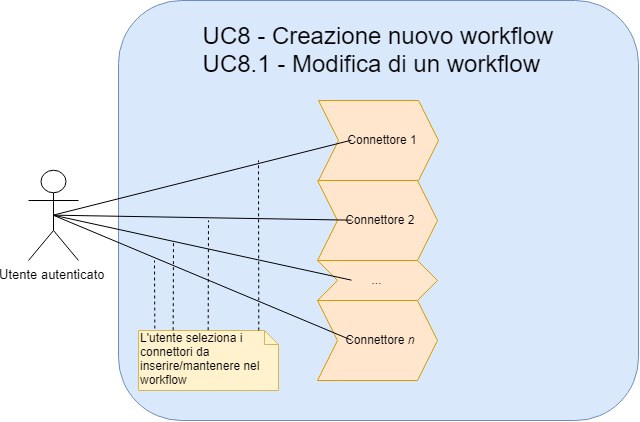
\includegraphics[width=13cm,keepaspectratio]{../includes/pics/Creazione_modifica_workflow.png}
	\caption{\label{fig:mission}Creazione e modifica di un \markg{workflow}}
\end{figure}
%\includegraphics[width=1\textwidth]{../includes/pics/Creazione_modifica_\markg{workflow}.png}

\subsubsection{UC8 - Creazione nuovo \markg{workflow}}
\begin{itemize}
	\item  Attori primari: utente autenticato;
	\item  Scopo e descrizione: l'utente crea un nuovo \markg{workflow};
	\item  Scenario principale:  
	\begin{enumerate}
		\item l'utente visualizza una lista di \markg{connettori} [UC9.3]-[UC9.17] che potrà inserire nel proprio \markg{workflow} personalizzato;
		\item sceglie quali \markg{connettori} aggiungere;
		\item imposta i \markg{connettori};
		\item sceglie l'ordine dei \markg{connettori};
		\item associa un comando vocale e\textbackslash o testuale associato all'avvio del \markg{workflow};
		\item salva il \markg{workflow} associandovi un nome o lasciando il nome di default.
	\end{enumerate}
	\item  Pre-condizione: l'utente vuole creare un nuovo \markg{workflow};
	\item  Post-condizione: l'utente ha creato un nuovo \markg{workflow} associato al proprio account.
\end{itemize}
\subsubsection{UC8.1 - Modifica \markg{workflow}}
\begin{itemize}
	\item  Attori primari: utente autenticato;
	\item  Scopo e descrizione: l'utente modifica un \markg{workflow} già creato;
	\item  Scenario principale:  
	\begin{enumerate}
		\item l'utente visualizza la lista di \markg{connettori} scelti [UC9.3]-[UC9.17];
		\item sceglie quali \markg{connettori} aggiungere, modificare o eventualmente eliminare;
		\item imposta i \markg{connettori} nuovi o modificati;
		\item può scegliere un nuovo ordine per i \markg{connettori};
		\item può associare un nuovo comando vocale e\textbackslash o testuale associato per l'avvio del \markg{workflow} che andrà a sostituire il vecchio comando;
		\item può modificare il nome associato al \markg{workflow} o lasciare il nome precedente.
	\end{enumerate}
	\item  Pre-condizione: l'utente vuole modificare un \markg{workflow};
	\item  Post-condizione: l'utente ha modificato un \markg{workflow} associato al proprio account.
\end{itemize}
\subsubsection{UC8.2 - Rimozione \markg{workflow}}
\begin{itemize}
	\item  Attori primari: utente autenticato;
	\item  Scopo e descrizione: l'utente elimina un \markg{workflow} già creato;
	\item  Scenario principale: l'utente visualizza la lista di \markg{workflow} associati al proprio account e tramite un comando elimina un determinato \markg{workflow} liberando anche il nome associato a quest'ultimo;
	\item  Pre-condizione: l'utente vuole rimuovere un \markg{workflow};
	\item  Post-condizione: l'utente ha rimosso un \markg{workflow} associato al proprio account.
\end{itemize}
\subsubsection{UC9 - Aggiunta \markg{connettore} generico}
\begin{itemize}
	\item  Attori primari: utente autenticato;
	\item  Scopo e descrizione: l'utente aggiunge un \markg{connettore} ad un \markg{workflow};
	\item  Scenario principale: l'utente visualizza la lista di \markg{connettori} proposti, dopo averne scelto uno imposta eventuali opzioni aggiuntive, il \markg{connettore} viene quindi aggiunto al \markg{workflow};
	\item  Pre-condizione: l'utente vuole aggiungere un \markg{connettore} al \markg{workflow};
	\item  Post-condizione: l'utente ha impostato il \markg{connettore} e questo è stato aggiunto al \markg{workflow} associato al proprio account.
\end{itemize}
\subsubsection{UC9.1 - Modifica \markg{connettore} generico}
\begin{itemize}
	\item  Attori primari: utente autenticato;
	\item  Scopo e descrizione: l'utente modifica un \markg{connettore} presente in un \markg{workflow};
	\item  Scenario principale: l'utente visualizza la lista di \markg{connettori} del \markg{workflow}, dopo averne scelto uno può modificare le opzioni aggiuntive dello stesso, il \markg{connettore} modificato viene quindi aggiunto al \markg{workflow} al posto del precedente;
	\item  Pre-condizione: l'utente vuole modificare un \markg{connettore} del \markg{workflow};
	\item  Post-condizione: l'utente ha impostato il \markg{connettore} e questo è stato aggiunto al \markg{workflow} sostituendo il vecchio \markg{connettore}.
\end{itemize}
\subsubsection{UC9.2 - Rimozione \markg{connettore} generico}
\begin{itemize}
	\item  Attori primari: utente autenticato;
	\item  Scopo e descrizione: l'utente modifica un \markg{workflow} rimuovendo uno o più \markg{connettori};
	\item  Scenario principale: l'utente visualizza la lista di \markg{connettori} del \markg{workflow}, tramite un apposito comando elimina uno o più \markg{connettori} presenti nel \markg{workflow} (eliminando tutti i \markg{connettori} può anche avvenire l'eliminazione del \markg{workflow} UC8.2);
	\item  Pre-condizione: l'utente vuole eliminare un \markg{connettore} dal \markg{workflow};
	\item  Post-condizione: l'utente ha modificato il \markg{workflow} eliminando il \markg{connettore} scelto.
\end{itemize}
\subsubsection{UC9.3 -\markg{Connettore}: messaggio di benvenuto}
\begin{itemize}
	\item  Attori primari: utente autenticato;
	\item  Scopo e descrizione: permette di impostare un messaggio di benvenuto associato al \markg{workflow} che si andrà a creare;
	\item  \markg{Voice flow} dell'assistente vocale: l'assistente comunica il testo scelto dall'utente come messaggio di benvenuto;
	\item  Pre-condizione: l'utente è autenticato, il sistema è funzionante e raggiungibile, si sta creando un \markg{workflow};
	\item  Post-condizione: l'utente ha impostato un messaggio di benvenuto per il \markg{workflow} corrente.
\end{itemize}

\begin{figure}[H]
	\centering
	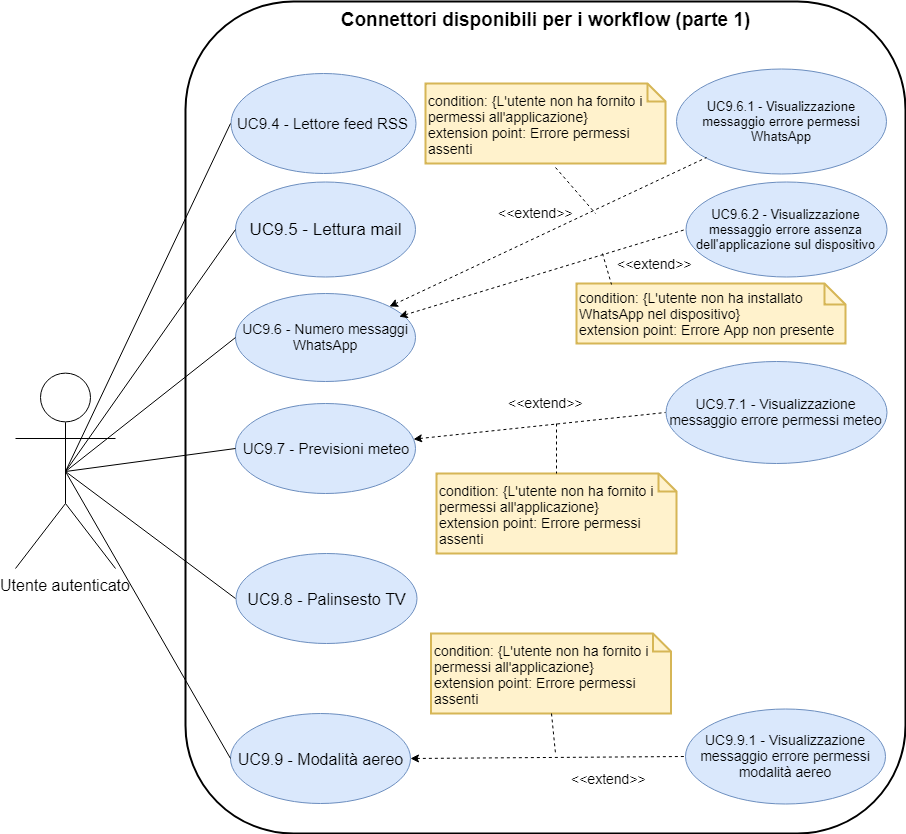
\includegraphics[width=15cm,keepaspectratio]{../includes/pics/wf1.png}
	\caption{\label{fig:mission}\markg{Connettori} disponibili [UC9.4] - [UC9.9]}
\end{figure}
%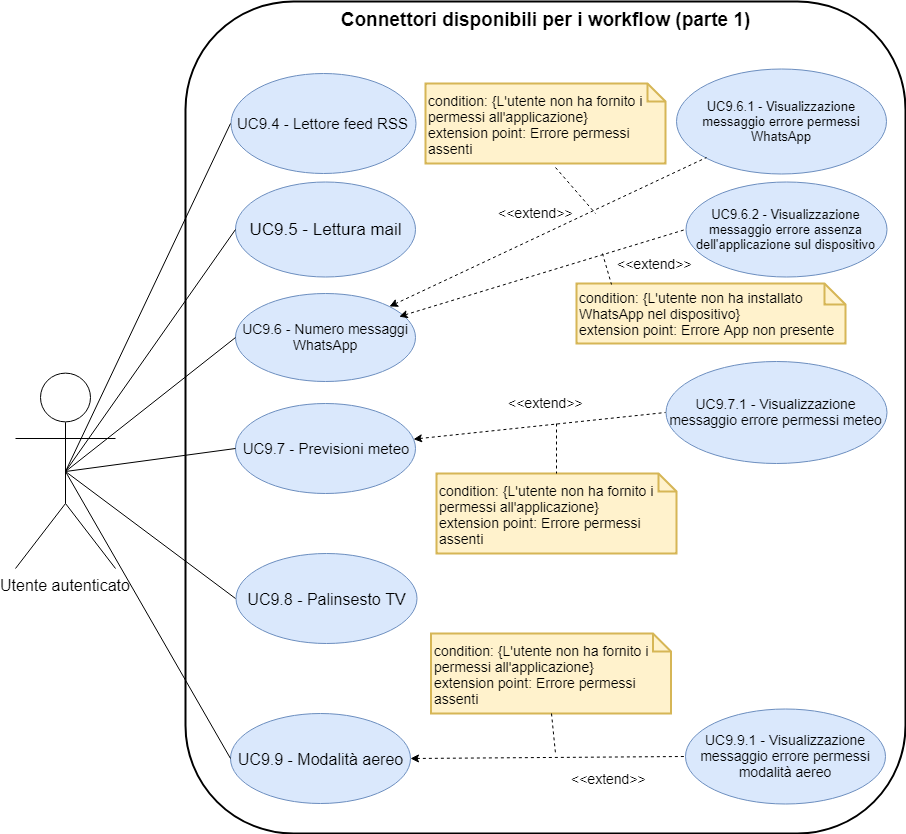
\includegraphics[width=1\textwidth]{../includes/pics/wf1.png}

\subsubsection{UC9.4 -\markg{Connettore}: lettore feed \markg{RSS}}
\begin{itemize}
	\item  Attori primari: utente autenticato;
	\item  Scopo e descrizione: permette all'assistente vocale di leggere un feed \markg{RSS} impostato dall'utente tramite URL, è inoltre possibile impostare un filtro per parole chiave [UC9.4.1];
	\item  \markg{Voice flow} dell'assistente vocale: l'assistente comunica il contenuto dell'ultimo feed \markg{RSS} ricevuto;
	\item  Pre-condizione: l'utente è autenticato, il sistema è funzionante e raggiungibile, si sta creando/modificando un \markg{workflow};
	\item  Post-condizione: l'utente ha impostato un \markg{connettore} che si occupa di leggere un feed \markg{RSS}.
\end{itemize}
\subsubsection{UC9.4.1 - Filtro feed \markg{RSS}}
\begin{itemize}
	\item  Attori primari: utente autenticato;
	\item  Scopo e descrizione: vengono presentate regole impostabili che fungono da criterio per filtrare feed \markg{RSS} di un \markg{connettore} per la lettura dei feed \markg{RSS};
	\item  \markg{Voice flow} dell'assistente vocale: l'assistente comunica il contenuto dell'ultimo feed \markg{RSS} filtrato secondo i criteri impostati;
	\item  Pre-condizione: il sistema è funzionante e raggiungibile, si sta creando/modificando un \markg{workflow}, nel \markg{workflow} corrente è presente un \markg{connettore} per la lettura di feed \markg{RSS};
	\item  Post-condizione: l'utente ha impostato dei criteri per filtrare un feed \markg{RSS}.
\end{itemize}
\subsubsection{UC9.5 -\markg{Connettore}: lettura mail}
\begin{itemize}
	\item  Attori primari: utente autenticato;
	\item  Scopo e descrizione: permette di associare un indirizzo di posta elettronica al \markg{connettore}, verranno estratti mittenti e titoli delle mail non aperte arrivate nelle ultime 24 ore;
	\item  \markg{Voice flow} dell'assistente vocale: l'assistente comunica titoli e mittenti delle mail marcate come non lette arrivate nelle ultime 24 ore;
	\item  Pre-condizione: l'utente è autenticato, il sistema è funzionante e raggiungibile, si sta creando/modificando un \markg{workflow};
	\item  Post-condizione: l'utente ha impostato un \markg{connettore} per ricevere \markg{feedback} vocali riferiti a una casella di posta elettronica.
\end{itemize}
\subsubsection{UC9.6 -\markg{Connettore}: lettura numero e mittenti di messaggi WhatsApp}
\begin{itemize}
	\item  Attori primari: utente autenticato;
	\item  Scopo e descrizione: \markg{connettore} non impostabile, se trova installato sul dispositivo WhatsApp, estrae numero di messaggi non letti e relativi mittenti;
	\item  \markg{Voice flow} dell'assistente vocale: l'assistente comunica, in ordine, numero di messaggi non letti e relativo mittente, per ogni mittente associato a messaggi non letti;
	\item  Estensioni:
		   \begin{itemize}
				\item se l'utente non fornisce all'applicazione i permessi necessari riceve un messaggio di errore [UC9.6.1];
				\item se l'utente non possiede WhatsApp come applicazione installata nel dispositivo, riceve un messaggio di errore [UC9.6.2].
		   \end{itemize}
	\item  Pre-condizione: l'utente è autenticato,il sistema è funzionante e raggiungibile, si sta creando/modificando un \markg{workflow};
	\item  Post-condizione: l'utente ha impostato un \markg{connettore} per ricevere \markg{feedback} vocali dei messaggi WhatsApp ricevuti.
\end{itemize}
\subsubsection{UC9.6.1 - Visualizzazione messaggio errore permessi WhatsApp}
\begin{itemize}
	\item  Attori primari: utente autenticato;
	\item  Scopo e descrizione: l'utente viene avvisato di non poter aggiungere il \markg{connettore} senza aver fornito i permessi necessari all'applicazione;
	\item  Scenario principale: l'utente visualizza l'errore relativo alla mancanza di permessi;
	\item  Pre-condizione: l'utente vuole aggiungere un \markg{connettore} senza aver fornito i permessi;
	\item  Post-condizione: l'utente è consapevole di dover fornire i permessi necessari per poter utilizzare il \markg{connettore}.
\end{itemize}
\subsubsection{UC9.6.2 - Visualizzazione messaggio errore assenza dell'applicazione WhatsApp sul dispositivo}
\begin{itemize}
	\item  Attori primari: utente autenticato;
	\item  Scopo e descrizione: l'utente viene avvisato della mancanza dell'applicazione WhatsApp sul dispositivo;
	\item  Scenario principale: l'utente visualizza l'errore relativo alla necessità di dover installare WhatsApp sul dispositivo per poter utilizzare il \markg{connettore};
	\item  Pre-condizione: l'utente vuole aggiungere un \markg{connettore} senza che WhatsApp sia installato sul dispositivo;
	\item  Post-condizione: l'utente è consapevole di dover installare l'applicazione per poter disporre del \markg{connettore} per la lettura di messaggi WhatsApp [UC9.6].
\end{itemize}
\subsubsection{UC9.7 -\markg{Connettore}: Meteo}
\begin{itemize}
	\item  Attori primari: utente autenticato;
	\item  Scopo e descrizione: permette di impostare una posizione tramite inserimento del nome di un comune o tramite geolocalizzazione del dispositivo \markg{Android}. Di questa posizione verranno comunicate le condizioni meteorologiche;
	\item  \markg{Voice flow} dell'assistente vocale: l'assistente comunica precipitazioni e temperature riferite alle 36 ore successive dell'area impostata dal \markg{connettore};
	\item  Estensioni: 
		   \begin{itemize}
				\item se l'utente non fornisce all'applicazione i permessi necessari riceve un messaggio di errore [UC9.7.1].
		   \end{itemize}
	\item  Pre-condizione: l'utente è autenticato, il sistema è funzionante e raggiungibile, si sta creando/modificando un \markg{workflow};
	\item  Post-condizione: l'utente ha impostato un \markg{connettore} per ricevere informazioni meteorologiche.
\end{itemize}
\subsubsection{UC9.7.1 - Visualizzazione messaggio errore permessi meteo}
\begin{itemize}
	\item  Attori primari: utente autenticato;
	\item  Scopo e descrizione: l'utente viene avvisato di non poter aggiungere il \markg{connettore} senza aver fornito i permessi necessari all'applicazione;
	\item  Scenario principale: l'utente visualizza l'errore relativo alla mancanza di permessi;
	\item  Pre-condizione: l'utente vuole aggiungere un \markg{connettore} meteo riferito alla posizione del dispositivo \markg{Android} senza aver fornito i permessi;
	\item  Post-condizione: l'utente è consapevole di dover fornire i permessi necessari per poter utilizzare il \markg{connettore}.
\end{itemize}
\subsubsection{UC9.8 -\markg{Connettore}: palinsesto TV}
\begin{itemize}
	\item  Attori primari: utente autenticato;
	\item  Scopo e descrizione: permette di selezionare alcuni canali in chiaro di cui si vuole sapere la programmazione, va inoltre specificata la fascia oraria;
	\item  \markg{Voice flow} dell'assistente vocale: l'assistente comunica, in ordine numerico, le trasmissioni dei canali scelti, che vanno in onda nella fascia oraria scelta;
	\item  Pre-condizione: l'utente è autenticato, il sistema è funzionante e raggiungibile, si sta creando/modificando un \markg{workflow};
	\item  Post-condizione: l'utente ha impostato un \markg{connettore} per ricevere informazioni su una parte del palinsesto televisivo.
\end{itemize}
\subsubsection{UC9.9 -\markg{Connettore}: imposta modalità aereo}
\begin{itemize}
	\item  Attori primari: utente autenticato;
	\item  Scopo e descrizione: \markg{connettore} non impostabile, permette di mettere in modalità aereo il dispositivo \markg{Android} su cui si sta eseguendo il sistema;
	\item  \markg{Voice flow} dell'assistente vocale: l'assistente comunica che il dispositivo è entrato in modalità aereo;
	\item  Estensioni: 
		   \begin{itemize}
				\item se l'utente non fornisce all'applicazione i permessi necessari riceve un messaggio di errore [UC9.9.1].
		   \end{itemize}
	\item  Pre-condizione: l'utente è autenticato, il sistema è funzionante e raggiungibile, si sta creando un \markg{workflow};
	\item  Post-condizione: l'utente ha impostato un \markg{connettore} che quando verrà eseguito porrà il dispositivo \markg{Android} in modalità aereo.
\end{itemize}
\subsubsection{UC9.9.1 - Visualizzazione messaggio errore permessi modalità aereo}
\begin{itemize}
	\item  Attori primari: utente autenticato;
	\item  Scopo e descrizione: l'utente viene avvisato di non poter aggiungere il \markg{connettore} senza aver fornito i permessi necessari all'applicazione;
	\item  Scenario principale: l'utente visualizza l'errore relativo alla mancanza di permessi;
	\item  Pre-condizione: l'utente vuole aggiungere un \markg{connettore} riferito all'attivazione della modalità aereo del dispositivo \markg{Android} senza aver fornito i permessi;
	\item  Post-condizione: l'utente è consapevole di dover fornire i permessi necessari per poter utilizzare il \markg{connettore}.
\end{itemize}

\begin{figure}[H]
	\centering
	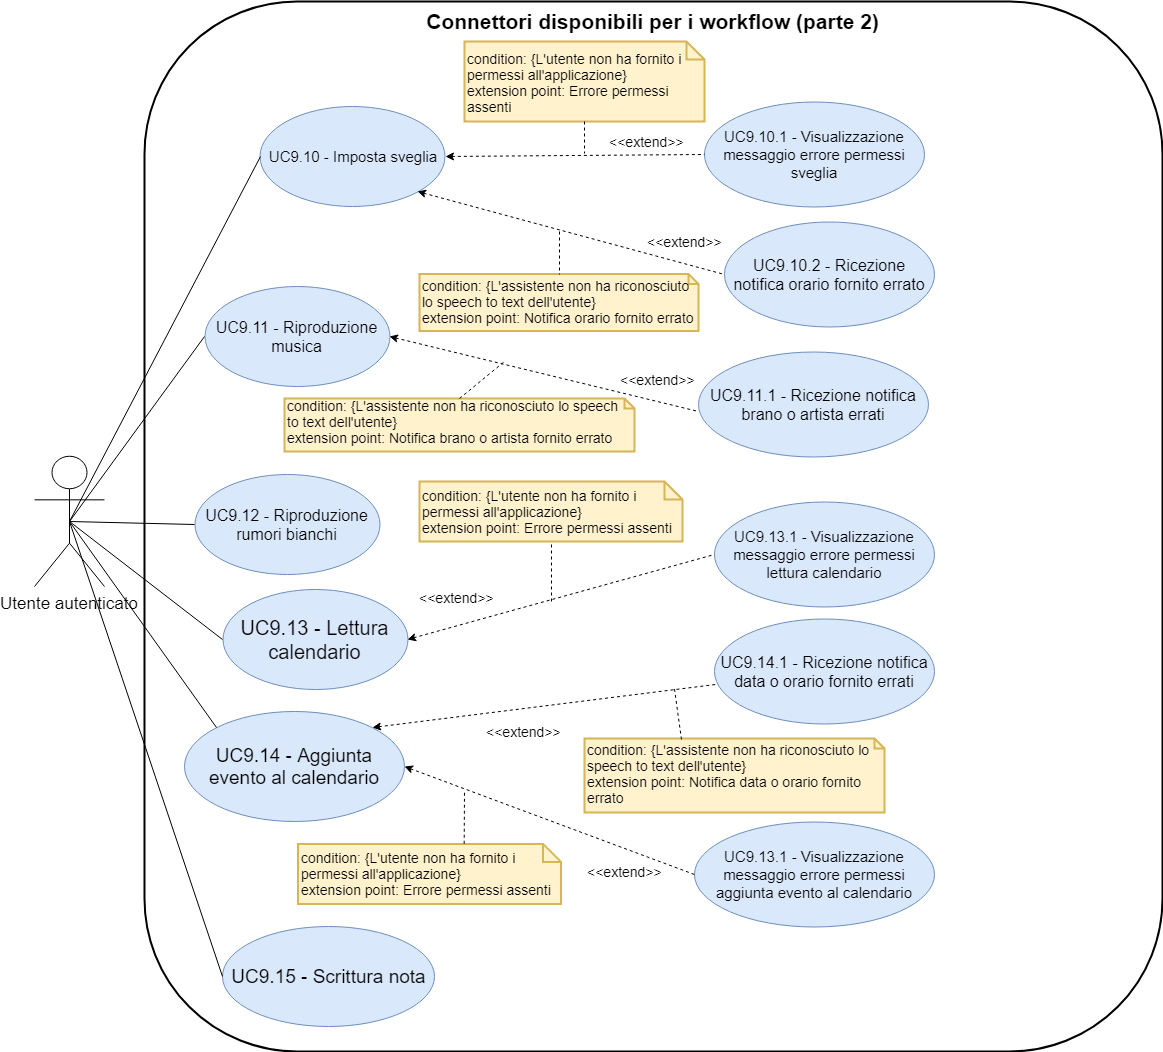
\includegraphics[width=15cm,keepaspectratio]{../includes/pics/wf2.png}
	\caption{\label{fig:mission}\markg{Connettori} disponibili [UC9.10] - [UC9.15]}
\end{figure}
%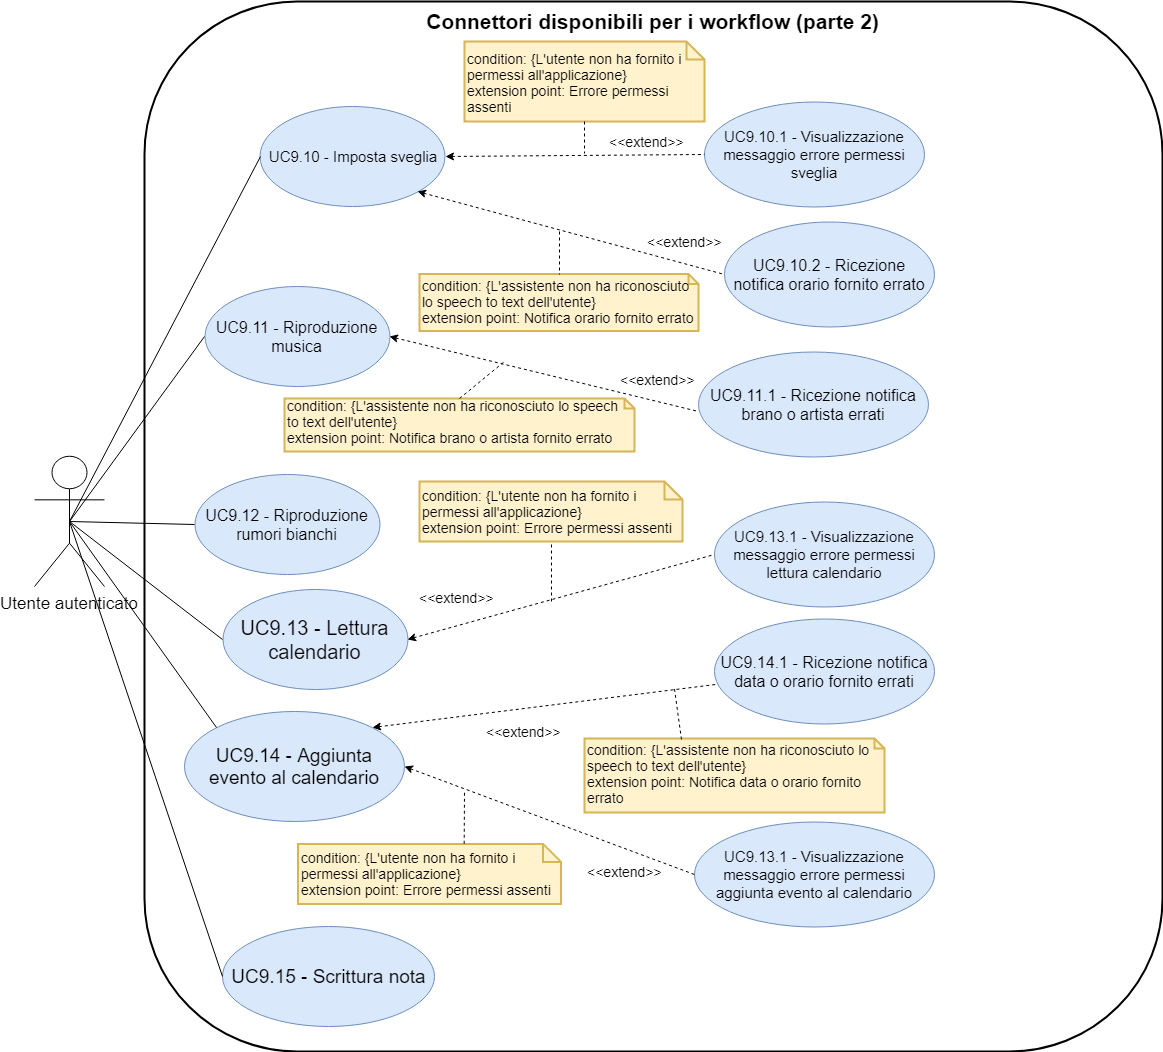
\includegraphics[width=1\textwidth]{../includes/pics/wf2.png}
\clearpage
\subsubsection{UC9.10 -\markg{Connettore}: imposta sveglia}
\begin{itemize}
	\item  Attori primari: utente autenticato;
	\item  Scopo e descrizione: permette di impostare un orario per la sveglia che verrà attivata alla chiamata del \markg{workflow} in cui questo \markg{connettore} è contenuto;
	\item  \markg{Voice flow} dell'assistente vocale: l'assistente chiede se c'e l'intenzione di impostare una sveglia, se la risposta e' positiva continua chiedendo l'orario da impostare;
	\item  Estensioni: 
		   \begin{itemize}
				\item se l'utente non fornisce all'applicazione i permessi necessari riceve un messaggio di errore [UC9.10.1];
				\item se l'utente durante lo \markg{speech-to-text} fornisce un orario errato riceve una notifica vocale [UC9.10.2].
		   \end{itemize}
	\item  Pre-condizione: l'utente è autenticato, il sistema è funzionante e raggiungibile, si sta creando/modificando un \markg{workflow};
	\item  Post-condizione: l'utente ha impostato un \markg{connettore} che quando verrà eseguito attiverà la sveglia sul dispositivo associato.
\end{itemize}
\subsubsection{UC9.10.1 - Visualizzazione messaggio errore permessi imposta sveglia}
\begin{itemize}
	\item  Attori primari: utente autenticato;
	\item  Scopo e descrizione: l'utente viene avvisato di non poter aggiungere il \markg{connettore} senza aver fornito i permessi necessari all'applicazione;
	\item  Scenario principale: l'utente visualizza l'errore relativo alla mancanza di permessi;
	\item  Pre-condizione: l'utente vuole aggiungere un \markg{connettore} riferito all'impostazione di una sveglia del dispositivo \markg{Android} senza aver fornito i permessi;
	\item  Post-condizione: l'utente è consapevole di dover fornire i permessi necessari per poter utilizzare il \markg{connettore}.
\end{itemize}
\subsubsection{UC9.10.2 - Ricezione notifica orario errato}
\begin{itemize}
	\item  Attori primari: utente autenticato;
	\item  Scopo e descrizione: l'utente tramite \markg{speech-to-text} ha fornito un orario errato;
	\item  Scenario principale: l'utente viene notificato della scelta errata dell'orario;
	\item  \markg{Voice flow} dell'assistente vocale: l'assistente notifica che l'utente ha impostato un orario sbagliato, comunica quindi se l'utente vuole reimpostare la sveglia;
	\item  Pre-condizione: l'utente ha scelto un orario errato;
	\item  Post-condizione: l'utente è consapevole di dover ripetere l'iterazione per impostare l'orario della sveglia.
\end{itemize}
\subsubsection{UC9.11 -\markg{Connettore}: riproduzione musica}
\begin{itemize}
	\item  Attori primari: utente autenticato;
	\item  Scopo e descrizione: permette di ascoltare un brano a scelta dell'utente;
	\item  \markg{Voice flow} dell'assistente vocale: l'assistente chiede all'utente il brano o l'artista che desisdera ascoltare, dopo aver ricevuto una risposta comincia la riproduzione musicale;
	\item  Estensioni:
		   \begin{itemize}
				\item se l'utente fornisce un titolo o un artista errato, riceve una notifica vocale [UC9.11.1].
		   \end{itemize}
	\item  Pre-condizione: l'utente è autenticato, il sistema è funzionante e raggiungibile, si sta creando/modificando un \markg{workflow};
	\item  Post-condizione: l'utente ha impostato un \markg{connettore} che quando verrà eseguito avvierà la riproduzione musicale dal dispositivo.
\end{itemize}
\subsubsection{UC9.11.1 - Ricezione notifica titolo o artista non riconosciuto}
\begin{itemize}
	\item  Attori primari: utente autenticato;
	\item  Scopo e descrizione: l'utente viene avvisato che il titolo o l'artista richiesto non è stato riconosciuto dall'assistente;
	\item  Scenario principale: l'utente riceve l'errore relativo all'errato riconoscimento da parte dell'assistente;
	\item  Pre-condizione: l'utente vuole aggiungere un \markg{connettore} al \markg{workflow} che permetta di avviare una riproduzione musicale specificando il titolo o l'artista;
	\item  Post-condizione: l'utente è consapevole di dover fornire il titolo o l'artista in un formato corretto per poter utilizzare il \markg{connettore}.
\end{itemize}
\subsubsection{UC9.12 -\markg{Connettore}: riproduzione \markg{rumori bianchi}}
\begin{itemize}
	\item  Attori primari: utente autenticato;
	\item  Scopo e descrizione: permette di impostare una durata di tempo, durante la quale, a \markg{workflow} chiamato, verrà riprodotta una \markg{playlist} di \markg{rumori bianchi};%in locale o da internet?
	\item  \markg{Voice flow} dell'assistente vocale: l'assistente riproduce la \markg{playlist} di suoni scelti;
	\item  Pre-condizione: l'utente è autenticato, il sistema è funzionante e raggiungibile, si sta creando/modificando un \markg{workflow};
	\item  Post-condizione: l'utente ha impostato un \markg{connettore} che quando verrà eseguito riprodurrà una \markg{playlist} di \markg{rumori bianchi}.
\end{itemize}
\subsubsection{UC9.13 -\markg{Connettore}: lettura calendario}
\begin{itemize}
	\item  Attori primari: utente autenticato;
	\item  Scopo e descrizione: permette, all'esecuzione, di ricevere informazioni sui prossimi eventi del calendario;
	\item  \markg{Voice flow} dell'assistente vocale: l'assistente comunica gli eventi del giorno segnati sul calendario; al termine chiede all'utente se vuole sapere quali sono gli eventi dei giorni successivi;
	\item  Estensioni: 
		   \begin{itemize}
				\item se l'utente non fornisce all'applicazione i permessi necessari riceve un messaggio di errore [UC9.13.1].
		   \end{itemize}
	\item  Pre-condizione: l'utente è autenticato,il sistema è funzionante e raggiungibile, si sta creando/modificando un \markg{workflow}, è stato impostato il periodo di tempo di cui si vogliono ricevere notizie sugli eventi e si sono forniti i permessi necessari;
	\item  Post-condizione: l'utente ha impostato un \markg{connettore} che quando verrà eseguito permetterà il riepilogo degli eventi in programma.
\end{itemize}
\subsubsection{UC9.13.1 - Visualizzazione messaggio errore permessi lettura calendario}
\begin{itemize}
	\item  Attori primari: utente autenticato;
	\item  Scopo e descrizione: l'utente viene avvisato di non poter aggiungere il \markg{connettore} senza aver fornito i permessi necessari all'applicazione.
	\item  Scenario principale: l'utente visualizza l'errore relativo alla mancanza di permessi.
	\item  Pre-condizione: l'utente vuole aggiungere un \markg{connettore} riferito alla lettura del calendario del dispositivo \markg{Android} senza aver fornito i permessi.
	\item  Post-condizione: l'utente è consapevole di dover fornire i permessi necessari per poter utilizzare il \markg{connettore}.
\end{itemize}
\subsubsection{UC9.14 -\markg{Connettore}: aggiunta evento calendario}
\begin{itemize}
	\item  Attori primari: utente autenticato;
	\item  Scopo e descrizione: permette, all'esecuzione, di aggiungere tramite \markg{speech-to-text} un evento al calendario;
	\item  \markg{Voice flow} dell'assistente vocale: l'assistente domanda se esiste l'intenzione di aggiungere un evento da parte dell'utente, a risposta positiva chiede di proseguire con la data ed eventuali informazioni dell'evento;
	\item  Estensioni: 
		   \begin{itemize}
			    \item se l'utente durante lo \markg{speech-to-text} imposta una data errata, riceve una notifica vocale [UC9.14.1];
				\item se l'utente non fornisce all'applicazione i permessi necessari riceve un messaggio di errore [UC9.14.2].
		   \end{itemize}
	\item  Pre-condizione: l'utente è autenticato,il sistema è funzionante e raggiungibile, si sta creando un \markg{workflow} e si sono forniti i permessi necessari;
	\item  Post-condizione: l'utente ha impostato un \markg{connettore} che quando verrà eseguito permetterà l'aggiunta di un evento al calendario \mark{Google}.
\end{itemize}
\subsubsection{UC9.14.1 - Ricezione notifica data errata}
\begin{itemize}
	\item  Attori primari: utente autenticato;
	\item  Scopo e descrizione: l'utente ha impostato una data sbagliata, può quindi decidere se modificare la data o eliminare l'aggiunta dell'evento;
	\item  Scenario principale: l'utente viene notificato dell'errata scelta della data;
	\item  \markg{Voice flow} dell'assistente vocale: l'assistente notifica che l'utente ha impostato una data sbagliata durante la fase di \markg{speech-to-text}, continua quindi chiedendo se desidera modificare la data o eliminare l'aggiunta dell'evento al calendario;
	\item  Pre-condizione: l'utente ha impostato una data sbagliata per un nuovo evento del calendario;
	\item  Post-condizione: l'utente è consapevole di non poter scegliere date errate e che può modificare la data o eliminare l'evento.
\end{itemize}
\subsubsection{UC9.14.2 - Visualizzazione messaggio errore permessi aggiunta evento calendario}
\begin{itemize}
	\item  Attori primari: utente autenticato;
	\item  Scopo e descrizione: l'utente viene avvisato di non poter aggiungere il \markg{connettore} senza aver fornito i permessi necessari all'applicazione;
	\item  Scenario principale: l'utente visualizza l'errore relativo alla mancanza di permessi;
	\item  Pre-condizione: l'utente vuole aggiungere un \markg{connettore} riferito all'aggiunta di un evento al calendario del dispositivo \markg{Android} senza aver fornito i permessi;
	\item  Post-condizione: l'utente è consapevole di dover fornire i permessi necessari per poter utilizzare il \markg{connettore}.
\end{itemize}
\subsubsection{UC9.15 -\markg{Connettore}: scrittura nota}
\begin{itemize}
	\item  Attori primari: utente autenticato;
	\item  Scopo e descrizione: permette, all'esecuzione, di aggiungere una nota al telefono tramite \markg{speech-to-text}, non vi è una limitazione alla lunghezza delle note;
	\item  \markg{Voice flow} dell'assistente vocale: l'assistente domanda se esiste l'intenzione di aggiungere una nuova nota da parte dell'utente, a risposta positiva chiede di proseguire con il corpo della nota;
	\item  Pre-condizione: l'utente è autenticato,il sistema è funzionante e raggiungibile, si sta creando/modificando un \markg{workflow} e sono stati forniti i permessi necessari;
	\item  Post-condizione: l'utente ha impostato un \markg{connettore} che quando verrà eseguito permetterà l'aggiunta di una nota.
\end{itemize}

\subsubsection{UC9.16 -\markg{Connettore}: Twitter}
\begin{itemize}
	\item  Attori primari: utente autenticato;
	\item  Scopo e descrizione: l'utente all'esecuzione può scegliere come interagire con Twitter, in particolare:
		   \begin{itemize}
				\item pubblicare un tweet [UC9.16.2];
				\item leggere gli ultimi tweet pubblicati da un singolo account [UC9.16.3];
				\item leggere gli ultimi tweet presenti nella bacheca personale [UC9.16.4].
		   \end{itemize}
	\item  \markg{Voice flow} dell'assistente vocale: l'assistente chiede all'utente in che modo vuole interagire con Twitter durante il \markg{workflow};
	\item  Estensioni: 
		   \begin{itemize}
				\item se l'utente non fornisce all'applicazione le credenziali d'accesso necessarie riceve un messaggio di errore [UC9.16.1.1];
				\item se l'utente fornisce all'applicazione il nome di un account errato, riceve un messaggio di errore [UC9.16.1.2];
				\item se l'utente durante lo \markg{speech-to-text} supera i 280 caratteri, riceve una notifica vocale [UC9.16.1.3].
		   \end{itemize}
	\item  Pre-condizione: l'utente è autenticato, il sistema è funzionante e raggiungibile, si sta creando un \markg{workflow}, si è associato un account Twitter e si sono forniti i permessi necessari;
	\item  Post-condizione: l'utente ha impostato un \markg{connettore} che quando verrà eseguito permetterà di interagire con Twitter durante il \markg{workflow}.
\end{itemize}

\begin{figure}[H]
	\centering
	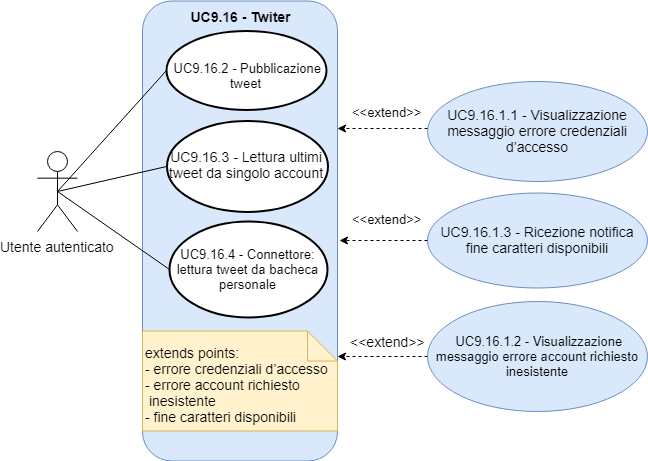
\includegraphics[width=14cm,keepaspectratio]{../includes/pics/connettore_twitter.png}
	\caption{\label{fig:mission}\markg{Connettore} Twitter}
\end{figure}
%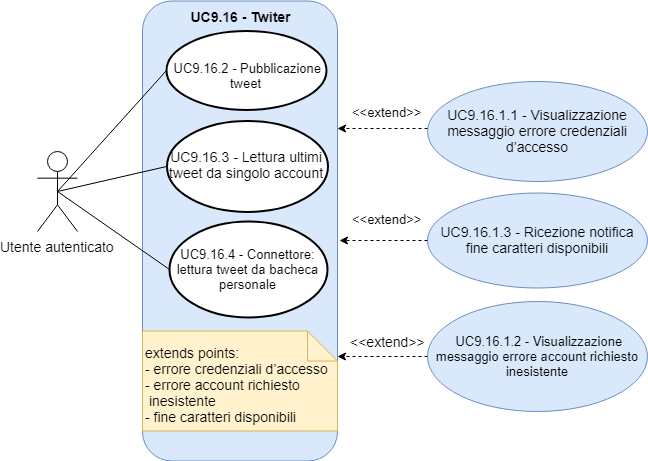
\includegraphics[width=1\textwidth]{../includes/pics/connettore_twitter.png}

\subsubsection{UC9.16.1.1 - Visualizzazione messaggio errore credenziali d'accesso}
\begin{itemize}
	\item  Attori primari: utente autenticato;
	\item  Scopo e descrizione: l'utente viene avvisato di non poter aggiungere il \markg{connettore} senza aver fornito le credenziali corrette per l'accesso all'account Twitter;
	\item  Scenario principale: l'utente visualizza l'errore relativo alla mancanza di credenziali d'accesso;
	\item  Pre-condizione: l'utente vuole aggiungere un \markg{connettore} riferito all'invio di tweet senza aver fornito le credenziali dell'account;
	\item  Post-condizione: l'utente è consapevole di dover fornire le credenziali corrette per poter utilizzare il \markg{connettore}.
\end{itemize}
\subsubsection{UC9.16.1.2 - Visualizzazione messaggio errore account Twitter richiesto inesistente}
\begin{itemize}
	\item  Attori primari: utente non autenticato;
	\item  Scopo e descrizione: l'utente viene avvisato che l'account inserito, di cui vuole ricevere i tweet pubblicati, non esiste;
	\item  Scenario principale: l'utente visualizza l'errore relativo all'errato inserimento del nome dell'account;
	\item  Pre-condizione: l'utente imposta il \markg{connettore} inserendo il nome errato di un account;
	\item  Post-condizione: l'utente è consapevole di dover fornire il nome di un account Twitter esistente.
\end{itemize}
\subsubsection{UC9.16.1.3 - Ricezione notifica fine caratteri disponibili}
\begin{itemize}
	\item  Attori primari: utente autenticato;
	\item  Scopo e descrizione: l'utente ha utilizzato tutti i 280 caratteri disponibili, può quindi decidere se inviare il messaggio, modificarlo o eliminarlo;
	\item  Scenario principale: l'utente viene notificato del raggiungimento del tetto limite di caratteri disponibili per il tweet;
	\item  \markg{Voice flow} dell'assistente vocale: l'assistente notifica che l'utente ha terminato la fase di \markg{speech-to-text}, continua quindi chiedendo se desidera: inviare il tweet, modificarlo facendo ricominciare lo \markg{speech-to-text} oppure eliminare completamente il corpo del tweet;
	\item  Pre-condizione: l'utente ha raggiunto il tetto massimo di caratteri impostati per il corpo di un tweet;
	\item  Post-condizione: l'utente è consapevole di non poter più aggiungere altro testo al tweet e che può inviare, modificare o eliminare il messaggio.
\end{itemize}
\subsubsection{UC9.16.2 - Pubblicazione tweet}
\begin{itemize}
	\item  Attori primari: utente autenticato;
	\item  Scopo e descrizione: permette, all'esecuzione, di pubblicare un tweet tramite \markg{speech-to-text}, testi più lunghi di 280 caratteri verranno troncati;
	\item  \markg{Voice flow} dell'assistente vocale: l'assistente chiede di ascoltare il corpo del tweet;
	\item  Pre-condizione: l'utente è autenticato,il sistema è funzionante e raggiungibile, si sta creando un \markg{workflow}, si è associato un account Twitter e si sono forniti i permessi necessari;
	\item  Post-condizione: l'utente ha impostato un \markg{connettore} che quando verrà eseguito permetterà la pubblicazione di un tweet.
\end{itemize}
\subsubsection{UC9.16.3 - Lettura ultimi tweet da singolo account}
\begin{itemize}
	\item  Attori primari: utente autenticato;
	\item  Scopo e descrizione: permette, all'esecuzione, di leggere gli ultimi tweet pubblicati da parte di un account. L'utente può durante l'ascolto scegliere di rispondere ad un tweet pubblicando una risposta [UC9.16.2];
	\item  \markg{Voice flow} dell'assistente vocale: l'assistente comunica che andrà a leggere i tweet dell'utente impostato, quindi ne comincia la lettura tramite text to speech. Nel caso l'utente voglia scrivere un tweet di risposta l'assistente chiede di proseguire dettando il corpo del tweet [UC9.16.2];
	\item  Pre-condizione: l'utente è autenticato,il sistema è funzionante e raggiungibile, si sta creando un \markg{workflow}, si è associato un account Twitter, è stato impostato l'account d e si sono forniti i permessi necessari;
	\item  Post-condizione: l'utente ha impostato un \markg{connettore} che quando verrà eseguito permetterà di ascoltare gli ultimi tweet di un certo utente prestabilito.
\end{itemize}
\subsubsection{UC9.16.4 -\markg{Connettore}: lettura tweet bacheca personale}
\begin{itemize}
	\item  Attori primari: utente autenticato;
	\item  Scopo e descrizione: permette, all'esecuzione, di leggere gli ultimi tweet presenti nella bacheca personale. L'utente può durante l'ascolto scegliere di rispondere ad un tweet pubblicando una risposta [UC9.16.2];
	\item  \markg{Voice flow} dell'assistente vocale: l'assistente comunica che andrà a leggere i tweet della bacheca personale dell'utente, ne comincia quindi la lettura tramite text to speech. Nel caso l'utente voglia scrivere un tweet di risposta l'assistente chiede di proseguire dettando il corpo del tweet [UC9.16.2];
	\item  Pre-condizione: l'utente è autenticato, il sistema è funzionante e raggiungibile, si sta creando/modificando un \markg{workflow};
	\item  Post-condizione: l'utente ha impostato un \markg{connettore} che quando verrà eseguito permetterà di ascoltare gli ultimi tweet della bacheca personale dell'utente.
\end{itemize}

\subsubsection{UC9.17 -\markg{Connettore}: \markg{Trello}}
\begin{itemize}
	\item  Attori primari: utente autenticato;
	\item  Scopo e descrizione: l'utente all'esecuzione può scegliere come interagire con \markg{Trello}, in particolare:
		   \begin{itemize}
				\item leggere le schede assegnate all'utente che sono presenti in una lista di una bacheca [UC9.17.2];
				\item creare una nuova scheda da aggiungere alla bacheca [UC9.17.3];
				\item spostare una scheda da una lista in un'altra lista della stessa bacheca [UC9.17.4].
		   \end{itemize}
	\item  \markg{Voice flow} dell'assistente vocale: l'assistente chiede all'utente in che modo vuole interagire con \markg{Trello} durante il \markg{workflow};
	\item  Estensioni: 
		   \begin{itemize}
				\item se l'utente non fornisce all'applicazione le credenziali d'accesso necessarie riceve un messaggio di errore [UC9.17.1.1];
				\item se l'utente fornisce all'applicazione il nome di una bacheca errata, riceve un messaggio di errore [UC9.17.1.2];
				\item se l'utente durante lo \markg{speech-to-text} fornisce il nome di una lista non presente nella bacheca, riceve una notifica vocale [UC9.17.1.3];
				\item se l'utente durante lo \markg{speech-to-text} fornisce il nome di una scheda non presente nella bacheca, riceve una notifica vocale [UC9.17.1.4].
		   \end{itemize}
	\item  Pre-condizione: l'utente è autenticato,il sistema è funzionante e raggiungibile, si sta creando/modificando un \markg{workflow}, si è associato un account \markg{Trello} e si sono forniti i permessi necessari;
	\item  Post-condizione: l'utente ha impostato un \markg{connettore} che quando verrà eseguito permetterà di interagire con \markg{Trello} durante il \markg{workflow}.
\end{itemize}

\begin{figure}[H]
	\centering
	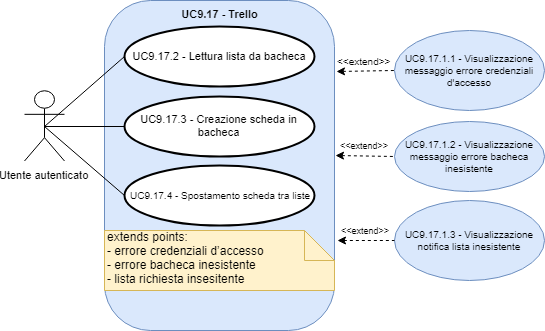
\includegraphics[width=14cm,keepaspectratio]{../includes/pics/trello.png}
	\caption{\label{fig:mission}\markg{Connettore} \markg{Trello}}
\end{figure}
%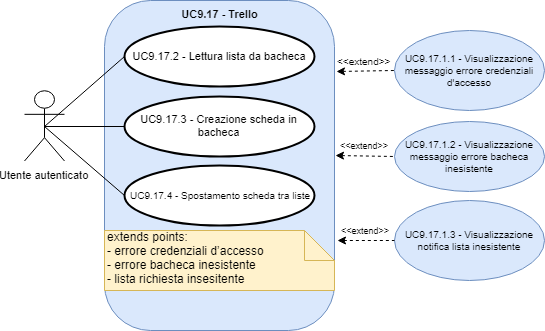
\includegraphics[width=1\textwidth]{../includes/pics/trello.png}

\subsubsection{UC9.17.1.1 - Visualizzazione messaggio errore credenziali d'accesso}
\begin{itemize}
	\item  Attori primari: utente autenticato;
	\item  Scopo e descrizione: l'utente viene avvisato di non poter aggiungere il \markg{connettore} senza aver fornito le credenziali corrette per l'accesso all'account \markg{Trello};
	\item  Scenario principale: l'utente visualizza l'errore relativo alla mancanza di credenziali d'accesso;
	\item  Pre-condizione: l'utente vuole aggiungere un \markg{connettore} riferito all'interazione con \markg{Trello} senza aver fornito le credenziali dell'account;
	\item  Post-condizione: l'utente è consapevole di dover fornire le credenziali corrette per poter utilizzare il \markg{connettore}.
\end{itemize}
\subsubsection{UC9.17.1.2 - Visualizzazione messaggio errore bacheca inesistente}
\begin{itemize}
	\item  Attori primari: utente autenticato;
	\item  Scopo e descrizione: l'utente viene avvisato che la bacheca inserita non risulta presente nell'account collegato;
	\item  Scenario principale: l'utente visualizza l'errore relativo all'errato inserimento del nome della bacheca;
	\item  Pre-condizione: l'utente imposta il \markg{connettore} inserendo il nome errato di una bacheca;
	\item  Post-condizione: l'utente è consapevole di dover fornire il nome di una bacheca presente tra quelle dell'account collegato.
\end{itemize}
\subsubsection{UC9.17.1.3 - Ricezione notifica lista inesistente}
\begin{itemize}
	\item  Attori primari: utente autenticato;
	\item  Scopo e descrizione: l'utente durante lo \markg{speech-to-text} ha scelto una lista che non è presente nella bacheca impostata nel \markg{connettore}, deve quindi scegliere di nuovo una lista da cui ricevere informazioni;
	\item  Scenario principale: l'utente viene notificato dell'assenza della lista richiesta;
	\item  \markg{Voice flow} dell'assistente vocale: l'assistente notifica che l'utente durante la fase di \markg{speech-to-text} ha fatto richiesta di una lista inesistente, continua quindi chiedendo se desidera cambiare la scelta della lista;
	\item  Pre-condizione: l'utente ha richiesto una lista non presente nella bacheca impostata nel \markg{connettore};
	\item  Post-condizione: l'utente è consapevole di aver richiesto una lista inesistente e che può modificare la sua richiesta.
\end{itemize}
\subsubsection{UC9.17.1.4 - Ricezione notifica scheda inesistente}
\begin{itemize}
	\item  Attori primari: utente autenticato;
	\item  Scopo e descrizione: l'utente durante lo \markg{speech-to-text} ha scelto una scheda che non è presente nella lista della bacheca impostata nel \markg{connettore}, deve quindi scegliere di nuovo una scheda su cui eseguire i comandi;
	\item  Scenario principale: l'utente viene notificato dell'assenza della scheda richiesta;
	\item  \markg{Voice flow} dell'assistente vocale: l'assistente notifica che l'utente durante la fase di \markg{speech-to-text} ha fatto richiesta di una scheda inesistente, continua quindi chiedendo se desidera cambiare la scelta della scheda;
	\item  Pre-condizione: l'utente ha richiesto una scheda non presente nella lista della bacheca impostata nel \markg{connettore};
	\item  Post-condizione: l'utente è consapevole di aver richiesto una scheda inesistente e che può modificare la sua richiesta.
\end{itemize}
\subsubsection{UC9.17.2 - Lettura lista da bacheca \markg{Trello}}
\begin{itemize}
	\item  Attori primari: utente autenticato;
	\item  Scopo e descrizione: permette, all'esecuzione, di leggere le prime schede assegnate all'utente di una lista facente parte di una bacheca a scelta dell'utente;
	\item  \markg{Voice flow} dell'assistente vocale: l'assistente domanda all'utente di quale lista desidera ricevere informazioni, dopo aver ricevuto risposta comincia la lettura tramite \markg{text-to-specch};
	\item  Pre-condizione: l'utente è autenticato, il sistema è funzionante e raggiungibile, si sta creando un \markg{workflow}, si è associato un account \markg{Trello} e si sono forniti i permessi necessari;
	\item  Post-condizione: l'utente ha impostato un \markg{connettore} che quando verrà eseguito permetterà di ascoltare il contenuto delle schede di una lista facente parte di una bacheca prestabilita.
\end{itemize}
\subsubsection{UC9.17.3 - Creazione scheda in bacheca \markg{Trello}}
\begin{itemize}
	\item  Attori primari: utente autenticato;
	\item  Scopo e descrizione: permette, all'esecuzione, di aggiungere una scheda ad una bacheca scelta precedentemente dall'utente;
	\item  \markg{Voice flow} dell'assistente vocale: l' assistente vocale domanda il nome della lista in cui l'utente vuole aggiungere la scheda, l'utente quindi comunica il corpo della scheda tramite \markg{speech-to-text};
	\item  Pre-condizione: l'utente è autenticato, il sistema è funzionante e raggiungibile, si sta creando un \markg{workflow}, si è associato un account \markg{Trello} e si sono forniti i permessi necessari;
	\item  Post-condizione: l'utente ha impostato un \markg{connettore} che quando verrà eseguito permetterà di aggiungere una nuova scheda ad una lista facente parte di una bacheca predefinita.
\end{itemize}
\subsubsection{UC9.17.4 - Spostamento scheda tra liste \markg{Trello}}
\begin{itemize}
	\item  Attori primari: utente autenticato;
	\item  Scopo e descrizione: permette, all'esecuzione, di spostare una scheda in un'altra lista facente parte di una bacheca scelta precedentemente dall'utente;
	\item  \markg{Voice flow} dell'assistente vocale: l'assistente vocale chiede il nome della lista da cui l'utente vuole spostare la scheda, il nome della scheda e il nome della lista su cui dovrà essere inserita la scheda;
	\item  Pre-condizione: l'utente è autenticato, il sistema è funzionante e raggiungibile, si sta creando/modificando un \markg{workflow}, si è associato un account \markg{Trello} e si sono forniti i permessi necessari;
	\item  Post-condizione: l'utente ha impostato un \markg{connettore} che quando verrà eseguito permetterà di spostare una scheda tra liste facenti parte di una bacheca prestabilita.
\end{itemize}

\subsubsection{UC10 - Attivazione vocale \markg{workflow}}
\begin{itemize}
	\item Attori primari: utente autenticato;
	\item Scopo e descrizione: l'utente vuole avviare un \markg{workflow};
	\item \markg{Voice flow} dell'assistente vocale: l'utente richiede tramite comando vocale all'assistente \markg{Amazon} \markg{Alexa} di avviare un \markg{workflow};
	\item Estensioni:
		se l'utente durante lo \markg{speech-to-text} fornisce il nome di un \markg{workflow} non presente nell'area personale dell'applicazione, riceve una notifica vocale [UC10.1].
	\item Pre-condizione: l'utente è autenticato, il sistema è funzionante e raggiungibile ed è stata avviata la skill relativa all'applicazione;
	\item Post-condizione: il \markg{workflow} richiesto dall'utente è stato avviato: viene eseguito il primo \markg{connettore}.
\end{itemize}

\subsubsection{UC10.1 - Ricezione notifica vocale \markg{workflow} inesistente}
\begin{itemize}
	\item Attori primari: utente autenticato;
	\item Scopo e descrizione: l'utente durante lo \markg{speech-to-text} ha scelto un \markg{workflow} non presente nell'area personale dell'applicazione;
	\item \markg{Voice flow} dell'assistente vocale: l'assistente notifica che l'utente durante la fase di \markg{speech-to-text} ha richiesto l'avvio di un \markg{workflow} inesistente;
	\item Pre-condizione: l'utente è autenticato ed ha richiesto l'avvio di un \markg{workflow} inesistente;
	\item Post-condizione: l'utente è a conoscenza di aver richiesto un \markg{workflow} non esistente.
\end{itemize}

\subsubsection{UC11 - Richiesta lista personale \markg{workflow}}
\begin{itemize}
	\item Attori primari: utente autenticato;
	\item Scopo e descrizione: l'utente vuole conoscere la sua lista personale di \markg{workflow};
	\item \markg{Voice flow} dell'assistente vocale: l'utente richiede tramite comando vocale all'assistente \markg{Amazon} \markg{Alexa} di elencare i suoi \markg{workflow} personali; l'assistente risponde leggendo la lista;
	\item Pre-condizione: l'utente è autenticato, il sistema è funzionante e raggiungibile ed è stata avviata la skill relativa all'applicazione;
	\item Post-condizione: l'utente conosce la lista di \markg{workflow} personali.
\end{itemize}

\subsubsection{UC12 - Richiesta aiuto}
\begin{itemize}
	\item Attori primari: utente autenticato;
	\item Scopo e descrizione: l'utente vuole ricevere un aiuto per utilizzare le funzionalità della skill;
	\item \markg{Voice flow} dell'assistente vocale: l'utente richiede un aiuto tramite comando vocale all'assistente \markg{Amazon} \markg{Alexa}; l'assistente elenca le azioni che l'utente può effettuare;
	\item Pre-condizione: l'utente è autenticato, il sistema è funzionante e raggiungibile ed è stata avviata la skill relativa all'applicazione;
	\item Post-condizione: l'utente conosce la lista di funzionalità della skill.
\end{itemize}

\subsubsection{UC13 - Richiesta di termine della \markg{skill}}
\begin{itemize}
	\item Attori primari: utente autenticato;
	\item Scopo e descrizione: l'utente vuole terminare la skill;
	\item \markg{Voice flow} dell'assistente vocale: l'utente richiede ad \markg{Amazon} \markg{Alexa} l'interruzione della skill corrente;
	\item Pre-condizione: l'utente è autenticato, il sistema è funzionante e raggiungibile ed è stata avviata la skill relativa all'applicazione;
	\item Post-condizione: la skill viene interrotta.
\end{itemize}

\subsubsection{UC14 - Richiesta di termine del \markg{connettore} corrente}
\begin{itemize}
	\item Attori primari: utente autenticato;
	\item Scopo e descrizione: l'utente vuole terminare il \markg{connettore} attualmente in esecuzione;
	\item \markg{Voice flow} dell'assistente vocale: l'utente richiede ad \markg{Amazon} \markg{Alexa} l'interruzione del \markg{connettore} corrente;
	\item Pre-condizione: l'utente è autenticato, il sistema è funzionante e raggiungibile ed è stata avviata la skill relativa all'applicazione;
	\item Post-condizione: il \markg{connettore} corrente viene interrotto e il \markg{workflow} procede con il \markg{connettore} seguente se presente.
\end{itemize}

\subsubsection{UC15 - Fallimento \markg{skill}}
\begin{itemize}
	\item  Attori primari: utente autenticato;
	\item  Scopo e descrizione: l'utente viene notificato che \markg{Amazon} \markg{Alexa} non è riuscita a eseguire un \markg{connettore};
	\item  Pre-condizione: l'utente ha avviato un \markg{workflow} e uno o più \markg{connettori} sono falliti;
	\item  Post-condizione: l'utente è notificato del fatto che \markg{Amazon} \markg{Alexa} non è riuscita a portare a termine uno o più \markg{connettori} del \markg{workflow} avviato.
\end{itemize}